\documentclass[english]{article}
\usepackage{graphicx}
\usepackage{amsmath}
\usepackage{hyperref}
\usepackage{setspace}
\usepackage{apacite}
\usepackage{hyperref}
\usepackage{natbib}
\usepackage{pxfonts}
\usepackage[utf8]{inputenc}
\usepackage[left=1in,right=1in,top=1in,bottom=1in]{geometry}
\usepackage[left]{lineno}
\usepackage{soul}
\linenumbers


\title{High-order cognition is supported by complex but compressible brain activity patterns} 

\author{Lucy L. W. Owen\textsuperscript{1, 2} and Jeremy R. Manning\textsuperscript{1,
*}\\\textsuperscript{1}Department of Psychological and Brain Sciences,\\Dartmouth College,
Hanover, NH\\[0.1cm]\textsuperscript{2}Carney Institute for Brain Sciences,\\Brown University,
Providence, RI\\[0.1cm] \textsuperscript{*}Address correspondence to
jeremy.r.manning@dartmouth.edu}

\begin{document}
\maketitle


\begin{abstract} 

We applied dimensionality reduction algorithms and pattern classifiers to
functional neuroimaging data collected as participants listened to a story,
temporally scrambled versions of the story, or underwent a resting state
scanning session. These experimental conditions were intended to require
different depths of processing and inspire different levels of cognitive
engagement. We considered two primary aspects of the data. First, we treated
the number of features (components) required to achieve a threshold decoding
accuracy as a proxy for the ``compressibility'' of the neural patterns (where
fewer components indicate greater compression). Second, we treated the
maximum achievable decoding accuracy across participants as an indicator of the
``stability'' of the recorded patterns. Overall, we found that neural patterns
recorded as participants listened to the intact story required fewer features
to achieve comparable classification accuracy to the other experimental
conditions. However, the peak decoding accuracy (achievable with more features)
was also highest during intact story listening. Taken together, our work
suggests that our brain networks flexibly reconfigure according to ongoing task
demands, and that the activity patterns associated with higher-order cognition
and high engagement are both more complex and more compressible than the
activity patterns associated with lower-order tasks and lower levels of
engagement.

\end{abstract}

\doublespacing

\section*{Introduction}

Large-scale networks, including the human brain, may be conceptualized as
occupying one or more positions along on a continuum. At one extreme, every
node is fully independent of every other node. At the other extreme, all nodes
behave identically. Each extreme optimizes key properties of how the network
functions. When every node is independent, the network is maximally
\textit{expressive}: if we define the network's ``state'' as the activity
pattern across its nodes, then every state is equally reachable by a network
with fully independent nodes. On the other hand, a network of identically
behaved nodes optimizes \textit{robustness}: any subset of nodes may be removed
from the network without any loss of function or expressive power, as long as
any single node remains. Presumably, most natural systems tend to occupy
positions between these extremes. We wondered: might the human brain
reconfigure itself to be more flexible or more robust according to ongoing
demands? In other words, might the brain reconfigure its connections or
behaviors under different circumstances to change its position along this
continuum?

% compression (redundancy) vs. complexity -- appear to balance each other, butnot necessarily. 

Closely related to the above notions of expressiveness versus robustness are
measures of how much \textit{information} is contained in a given signal or
pattern, and how \textit{redundant} a signal is~\citep{Shan48}. Formally,
information is defined as the amount of uncertainty about a given variables'
outcomes (i.e., entropy), measured in \textit{bits}, or the optimal number of
yes/no questions needed to reduce uncertainty about the variable's outcomes to
zero. Highly complex systems with many degrees of freedom (i.e., high
flexibility and expressiveness), are more information-rich than simpler or more
constrained systems. The redundancy of a signal denotes the difference how
expressive the signal \textit{could} be (i.e., proportional to the number of
unique states or symbols used to transmit the signal) and the actual
information rate (i.e., the entropy of each individual state or symbol). If a
brain network's nodes are fully independent, then the number of bits required
to express a single activity pattern is proportional to the number of nodes.
The network would also be minimally redundant, since the status of every node
would be needed to fully express a single brain activity pattern. If a brain
network's nodes are fully coupled and identical, then the number of bits
required to express a single activity pattern is proportional to the number of
unique states or values any individual node can take on. Such a network would
be highly redundant, since knowing any individual node's state would be
sufficient to recover the full-brain activity pattern. Highly redundant systems
are also robust, since there is little information loss from losing any given
observation.

We take as a given that brain activity is highly flexible: our brains can
exhibit nearly infinite activity patterns. This flexibility implies that our
brains activity patterns are highly information rich. However, brain activity
patterns are also highly structured. For example, full-brain correlation
matrices are stable within~\citep{FinnEtal15, FinnEtal17, GratEtal18} and
across~\citep{YeoEtal11, GlerEtal12, GratEtal18, ColeEtal14} individuals. This
stability suggests that our brains' activity patterns are at least partially
constrained, for example by anatomical, external, or internal factors.
Constraints on brain activity that limit its flexibility decrease
expressiveness (i.e., its information rate). However, constraints on brain
activity also increase its robustness to noise (e.g., ``missing'' or corrupted
signals may be partially recovered). For example, recent work has shown that
full-brain activity patterns may be reliably recovered from only a relatively
small number of implanted electrodes~\citep{OwenEtal20, ScanEtal21}. This
robustness property suggests that the relevant signal (e.g., underlying factors
that have some influence over brain activity patterns) are compressible.

\begin{figure}[tp]

  \centering
  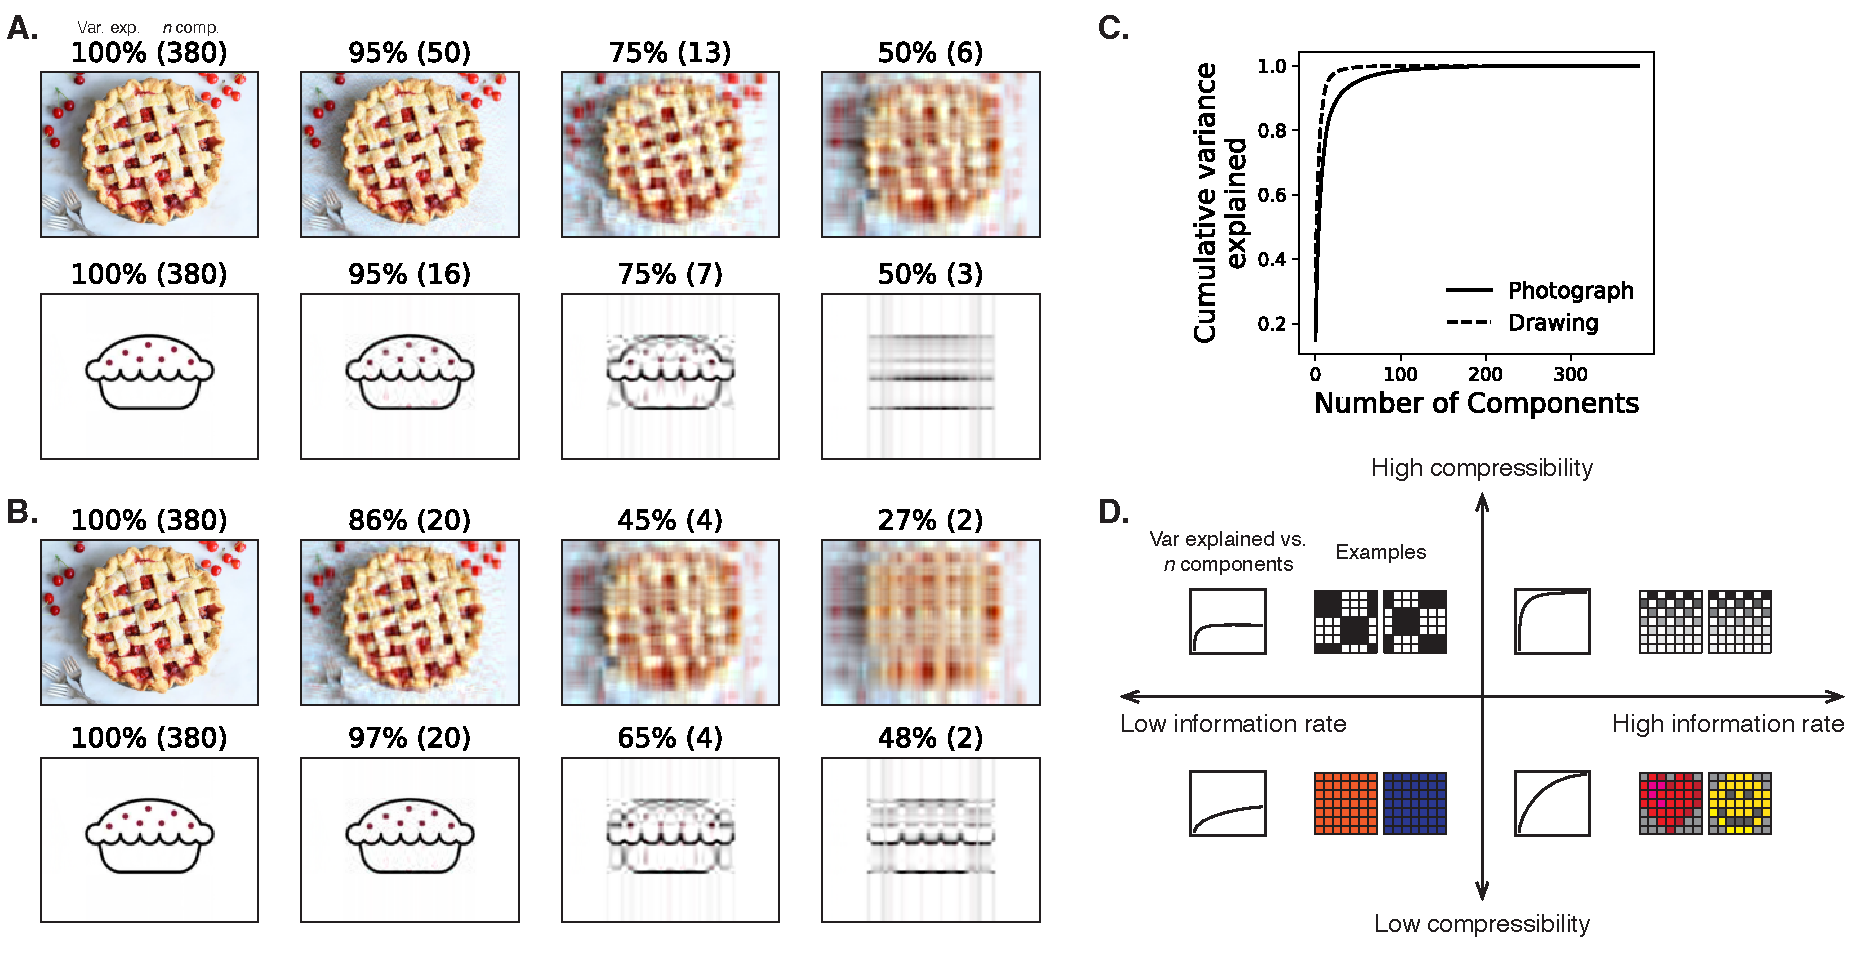
\includegraphics[width=\textwidth]{figs/information_and_compressibility}
  
  \caption{\textbf{Information content and compressibility.} \textbf{A. Variance
  explained for two images.} We applied principal components analysis to a
  photograph and drawing, treating each row of the images as ``observations.''
  Across columns, we identified the number of components required to explain
  100\%, 95\%, 75\%, or 50\% of the cumulative variance in each image (the 100\%
  columns denote the original images). The numbers of components are indicate in
  parentheses, and the resulting ``compressed'' images are displayed. \textbf{B.
  Representing two images with different numbers of components.} Using the same
  principal component decompositions as in Panel A, we computed the cumulative
  proportion of variance explained with 380 (original images), 20, 4, or 2
  components. \textbf{C. Cumulative variance explained versus number of
  components.} For the images displayed in Panels A and B, we plot the cumulative
  proportion of variance explained as a function of the number of components used
  to represent each image. \textbf{D. Information rate and compressibility.}
  Across multiple images, the information rate (i.e., the amount of information
  contained in each image; horizontal axis) is high when each individual pixel
  provides information that cannot be inferred from other pixels.
  High-information rate images tend to be high-resolution, and low-information
  rate images tend to be low-resolution. Compressibility is related to the
  difference between the information required to specify the original versus
  compressed images (vertical axis). Highly compressible images often contain
  predictable structure (redundancies) that can be leveraged to represent the
  images much more efficiently than in their original feature spaces.}
  
  \label{fig:information-compression} 
  \end{figure}

To the extent that brain activity patterns contain rich task-relevant
information, we should be able to use the activity patterns to accurately
differentiate between different aspects of the task~\citep[e.g., using pattern
classifiers;][]{NormEtal06b}. For example, prior work has shown a direct
correspondence between classification accuracy and the information content of a
signal~\citep{Alva02}. To the extent that brain activity patterns are
compressible, we should be able to generate simplified (e.g., lower
dimensional) representations of the data while still preserving the relevant or
important aspects of the original signal. In general, information content and
compressibility are related but are partially dissociable
(Fig.~\ref{fig:information-compression}). If a given signal (e.g., a
representation of brain activity patterns) contains more information about
ongoing cognitive processes, then the peak decoding accuracy should be high.
And if the signal is compressible, a low-dimensional embedding of the signal
will be similarly informative to the original signal
(Fig.~\ref{fig:information-compression}D).


Several recent studies suggest that the complexity of brain activity is
task-dependent, whereby simpler tasks with lower cognitive demands are
reflected by simpler and more compressible brain activity patterns, and more
complex tasks with higher cognitive demands are reflected by more complex and
less compressible brain activity patterns~\citep{MackEtal20, OwenEtal21}. These
findings complement other work suggesting that functional connectivity
(correlation) patterns are task-dependent~\citep{FinnEtal17, OwenEtal20,
ColeEtal14}, although see~\cite{GratEtal18}. Higher-order cognitive processing
of a common stimulus also appears to drive more stereotyped task-related
activity and functional connectivity across individuals~\citep{HassEtal08,
LernEtal11, SimoChan20, SimoEtal16}.

The above prior studies are consistent with two potential descriptions of how
cognitive processes are reflects in brain activity patterns. One possibility is
that the information rate of brain activity increases during more complex or
higher-level cognitive processing. If so, then the ability to reliably decode
cognitive states from brain activity patterns should improve with task
complexity or with the level (or ``depth'') of cognitive processing. A second
possibility is that the compressibility of brain activity patterns increases
during more complex or higher-level cognitive processing. If so, then
individual features of brain recordings, or compressed representations of brain
recordings, should carry more information during complex or high-level (versus
simple or low-level) cognitive tasks.

We used a previously collected neuroimaging dataset to estimate the extent to
which each of these two possibilities might hold. The dataset we examined
comprised functional magnetic resonance imaging (fMRI) data collected as
participants listened to an audio recording of a 10-minute story, temporally
scrambled recordings of the story, or underwent a resting state
scan~\citep{SimoEtal16}. Each of these experimental conditions evokes different
depths of cognitive processing~\citep{SimoEtal16,LernEtal11,
HassEtal08,OwenEtal21}. We used across-participant classifiers to decode
listening times in each condition, as a proxy for how ``informative'' the
task-specific activity patterns were~\citep{SimoChan20}. We also use principle
components analysis to generate lower-dimensional representations of the
activity patterns. We then repeated the classification analyses after
preserving different numbers of components and examined how classification
accuracy changed across the different experimental conditions.



\section*{Results}

\begin{figure}
  \centering
  
  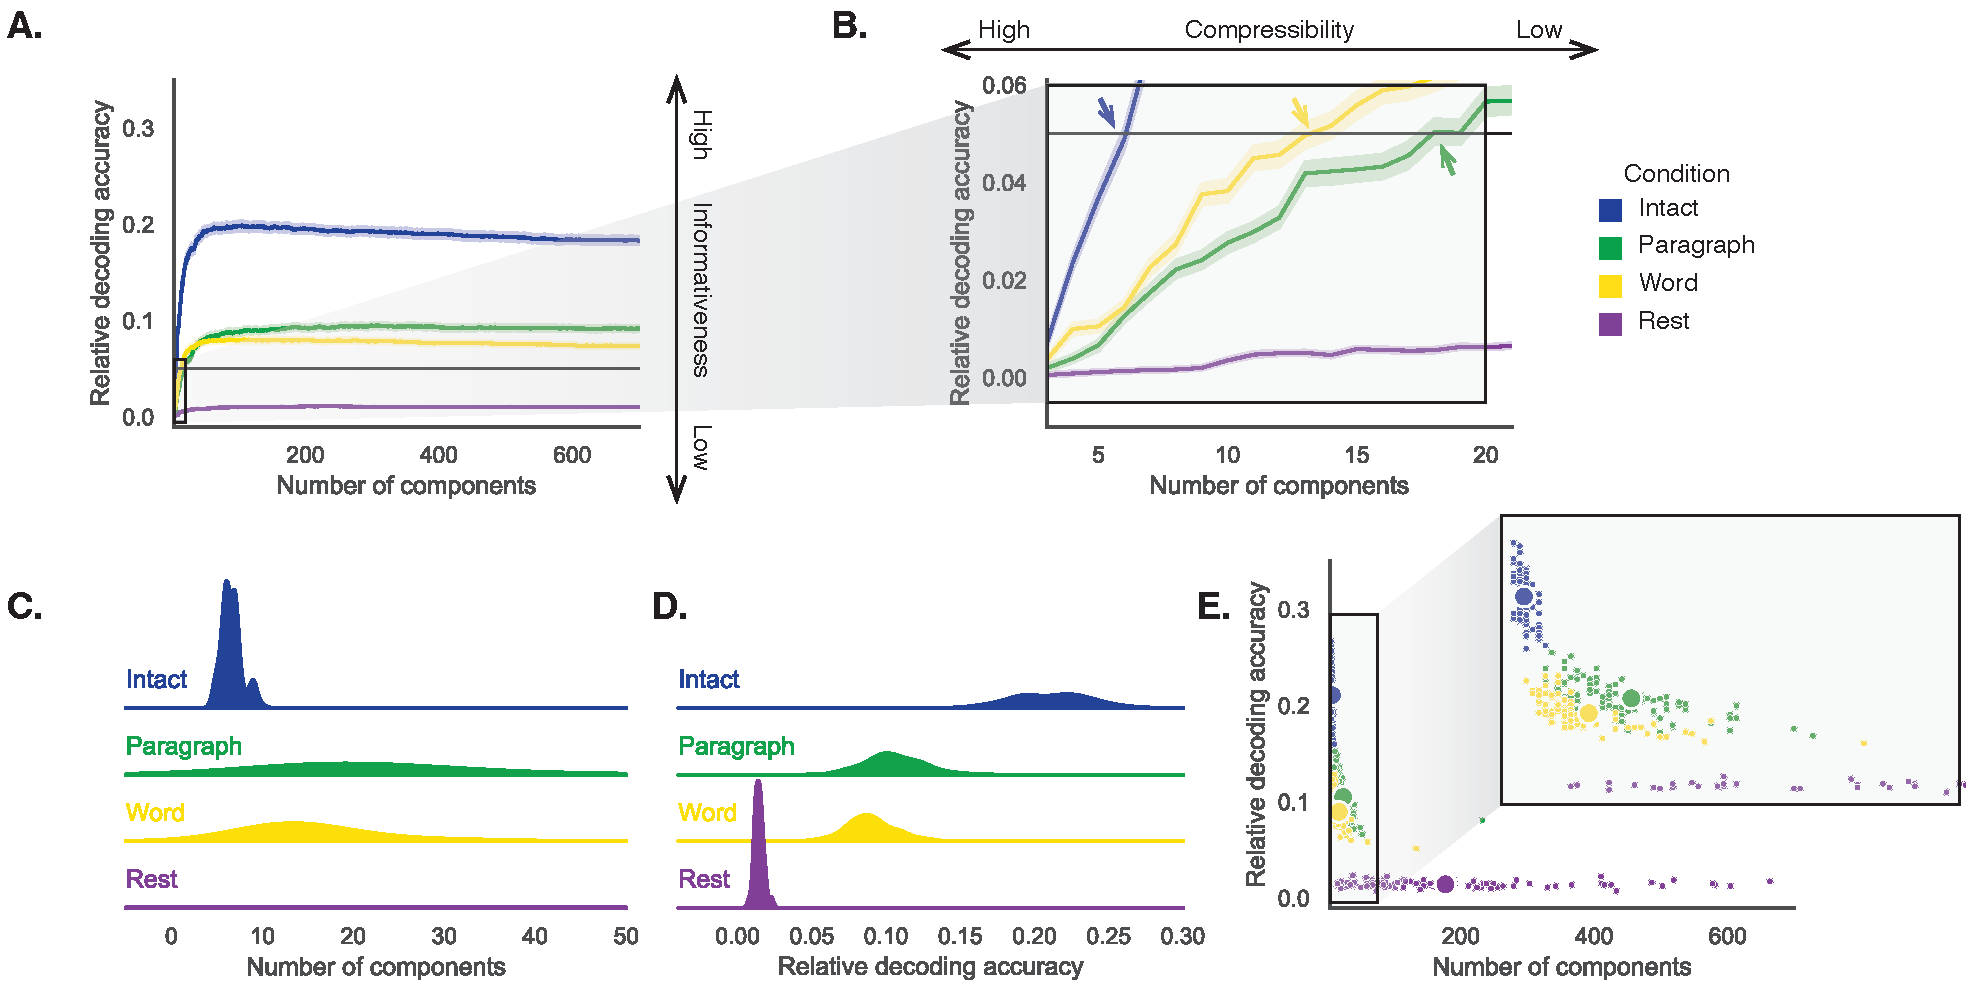
\includegraphics[width=0.8\textwidth]{figs/decoding_and_inflection}

  \caption{\textbf{Decoding accuracy and compression.} \textbf{A. Decoding accuracy by
      number of components.} Ribbons of each color display
    cross-validated decoding performance for each condition (intact,
    paragraph, word, and rest), as a function of the number of components (features) used to
    represent the data.  The horizontal red line denotes chance performance, and the horizontal black
    line denotes 5\% decoding accuracy (used as a reference in Panel B).  \textbf{B. Numbers of components
    required to reach a fixed decoding accuracy threshold, by condition.}  The panel displays a zoomed-in
    view of the inset in Panel A.  Intersections between each condition's decoding accuracy curve
    and the 5\% decoding accuracy reference line are marked by arrows.  \textbf{C. Estimating
    inflection points.}  We sought to identify an ``inflection point'' for each decoding curve, denoting
    the number of components at which the decoding curve asymptotes.  We fit sigmoid functions to each
    decoding curve (left sub-panel) and then computed the minimum number of components where the
    second derivative of the sigmoid was both positive and less than a threshold value of 0.0001.
    \textbf{D. Inflection points by condition.}  Each dot displays the number of components ($x$-axis)
    and decoding accuracy ($y$-axis) at one condition's inflection point.}

    \label{fig:decoding-inflection}
  \end{figure}





\begin{figure}
  \centering
  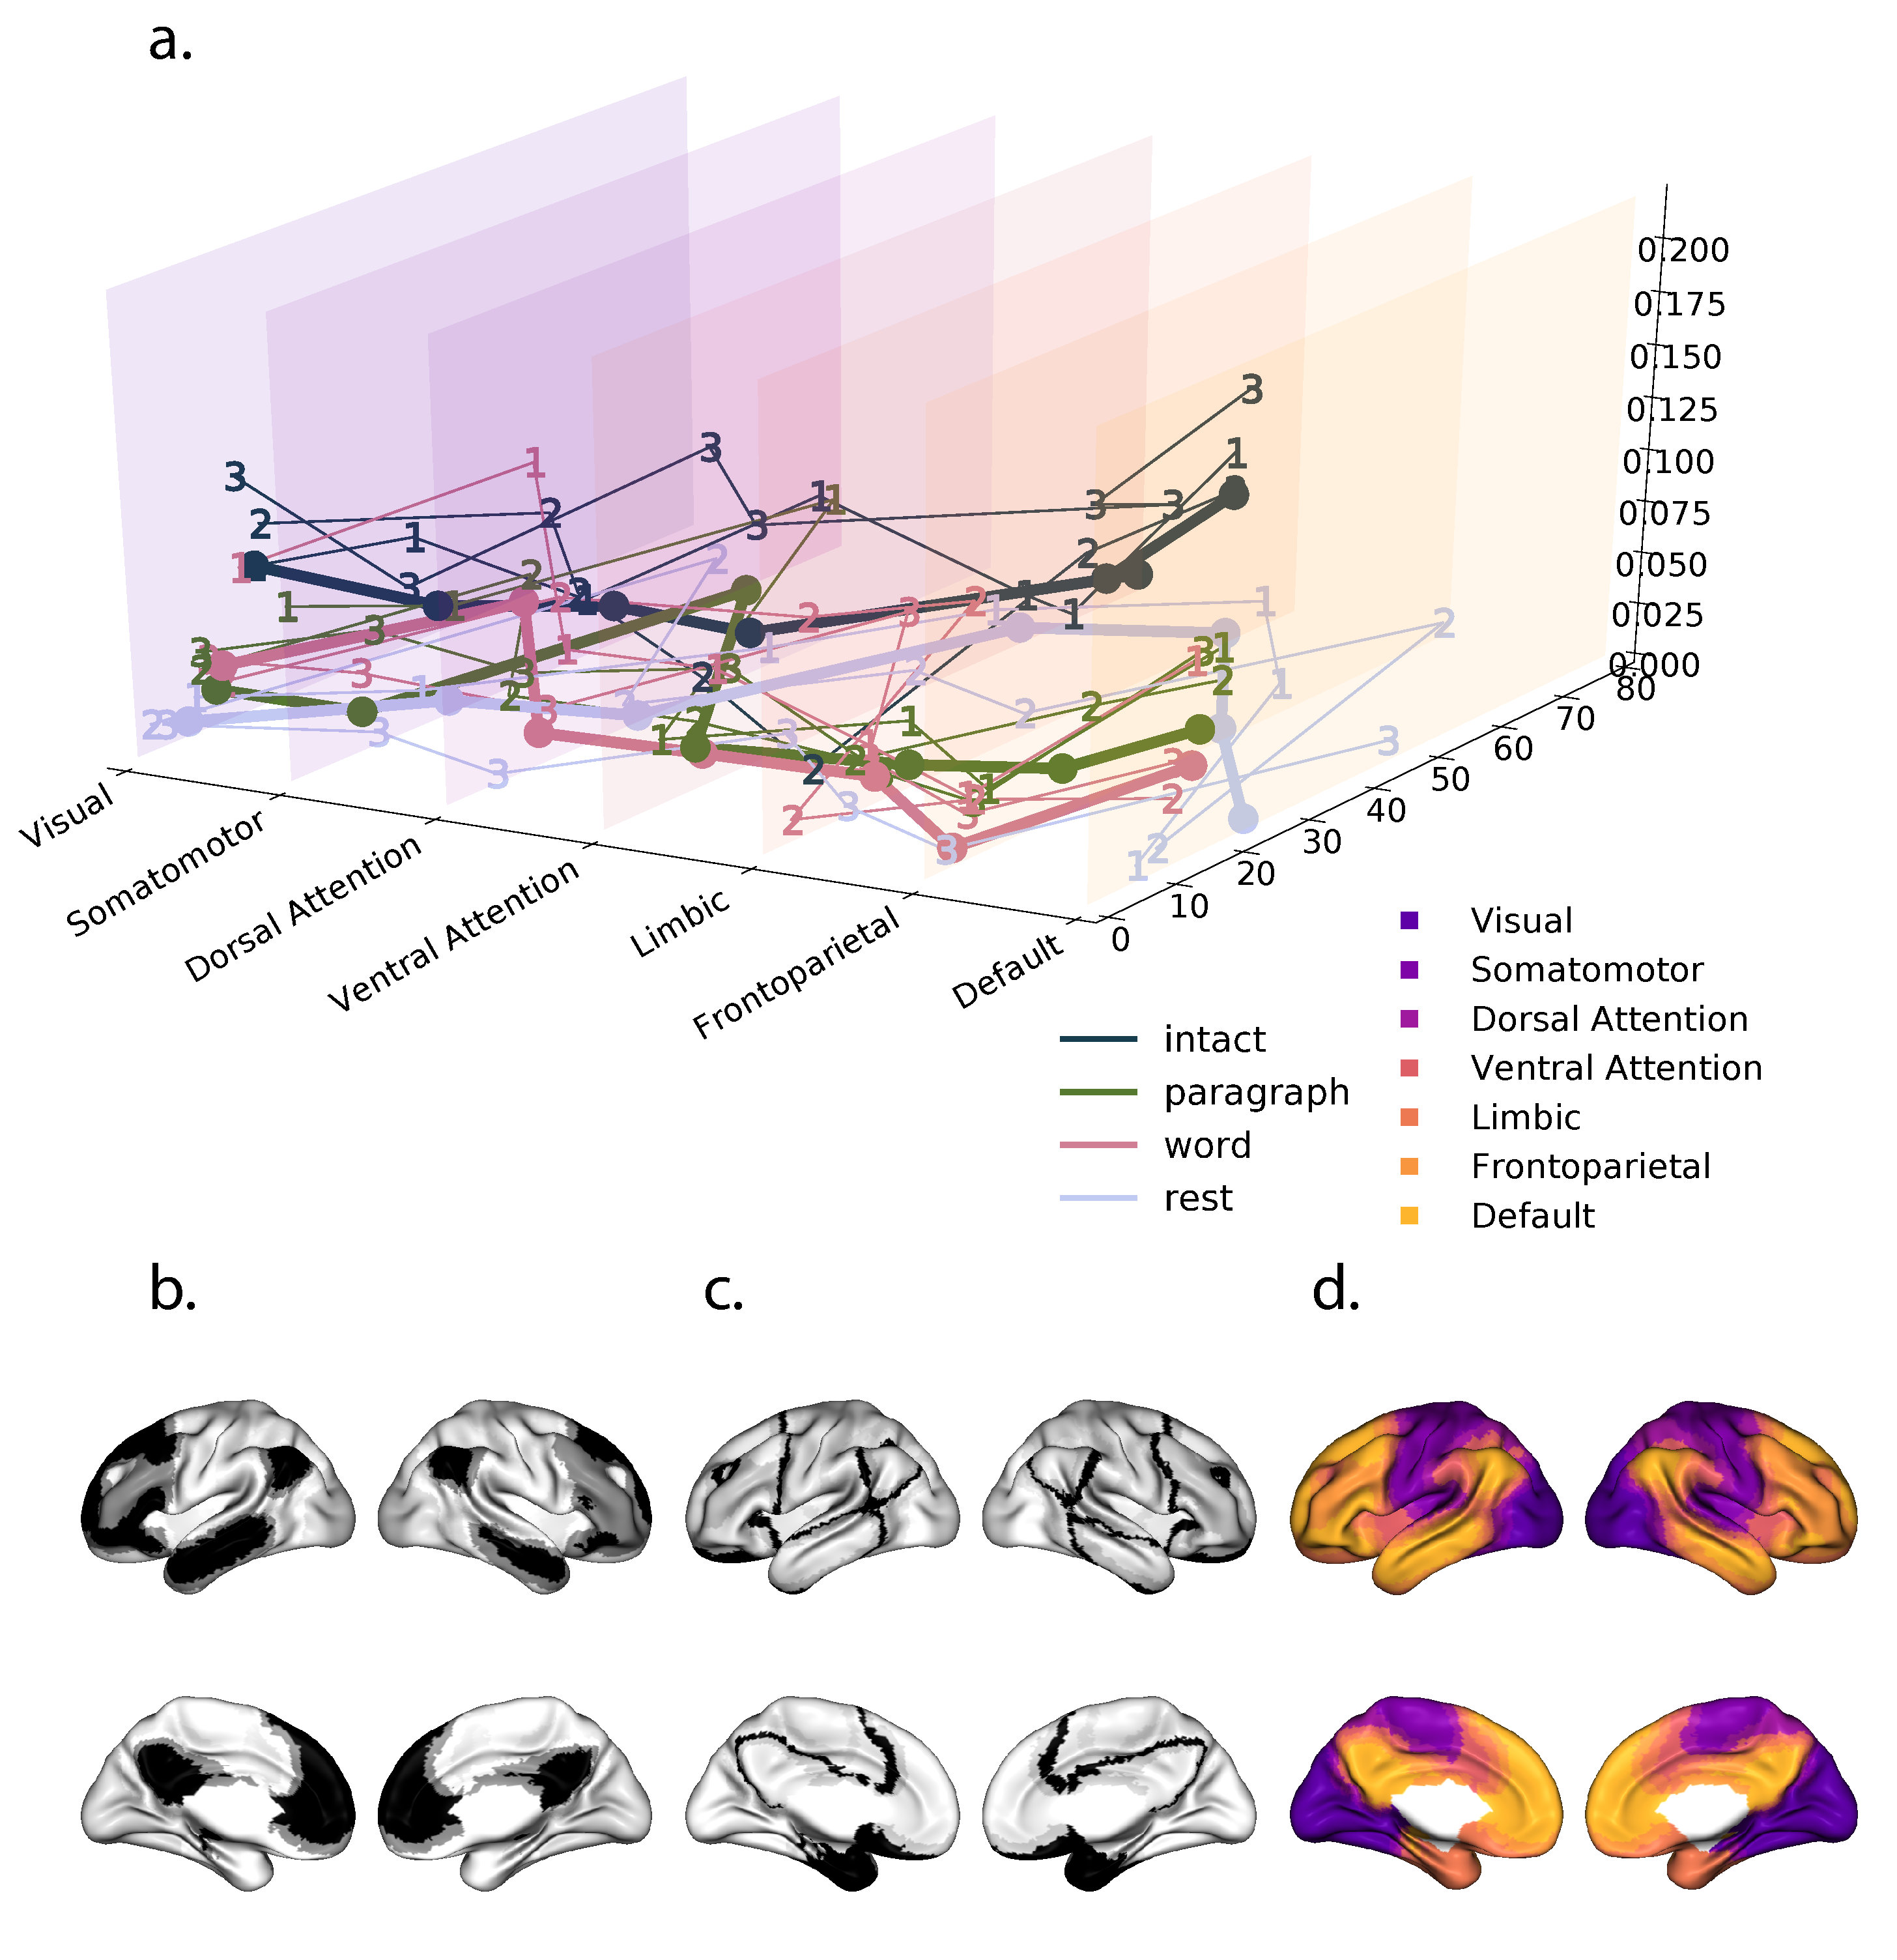
\includegraphics[width=0.8\textwidth]{figs/decode_pcs_network}
  \caption{\textbf{Inflection points by network.} \textbf{a.}
    Inflection point was calculated as explained in
    Fig.~\ref{fig:decode_interpret}, b. Analyses were limited by the
    brain networks (using the \cite{YeoEtal11} network parcellation) and
    arranged in increasing order relative to the intact condition.
    \textbf{b. and c.} For the total time in the intact condition, we are plotting the relative inflection points (\textbf{b.}) and corresponding number of components (\textbf{c.}) by network. \textbf{d.} The network parcellation defined by \cite{YeoEtal11} is displayed on the inflated brain maps. The colors and network labels serve as a legend for \textbf{a.} and \textbf{d.}}
  \label{fig:networks}
\end{figure}

We also wondered how this compression would change across brain regions.  We repeated the analysis but limited the brain hubs to 7 networks using the Yeo et al. (2011) network parcellation shown here in the inflated brain (Fig.~\ref{fig:decode_pcs_network}, d.). We found that as complexity of the stimuli increases, decoding accuracy increases
with higher cognitive areas. (Fig.~\ref{fig:decode_pcs_network}).


% As complexity of the stimuli increases, decoding accuracy increases
% with higher cognitive areas. (Fig.~\ref{fig: decode_pcs_network}).

%  If, there is some understanding of the narrative that accumulates over time, we should be able to see that change.

\begin{figure}
  \centering
  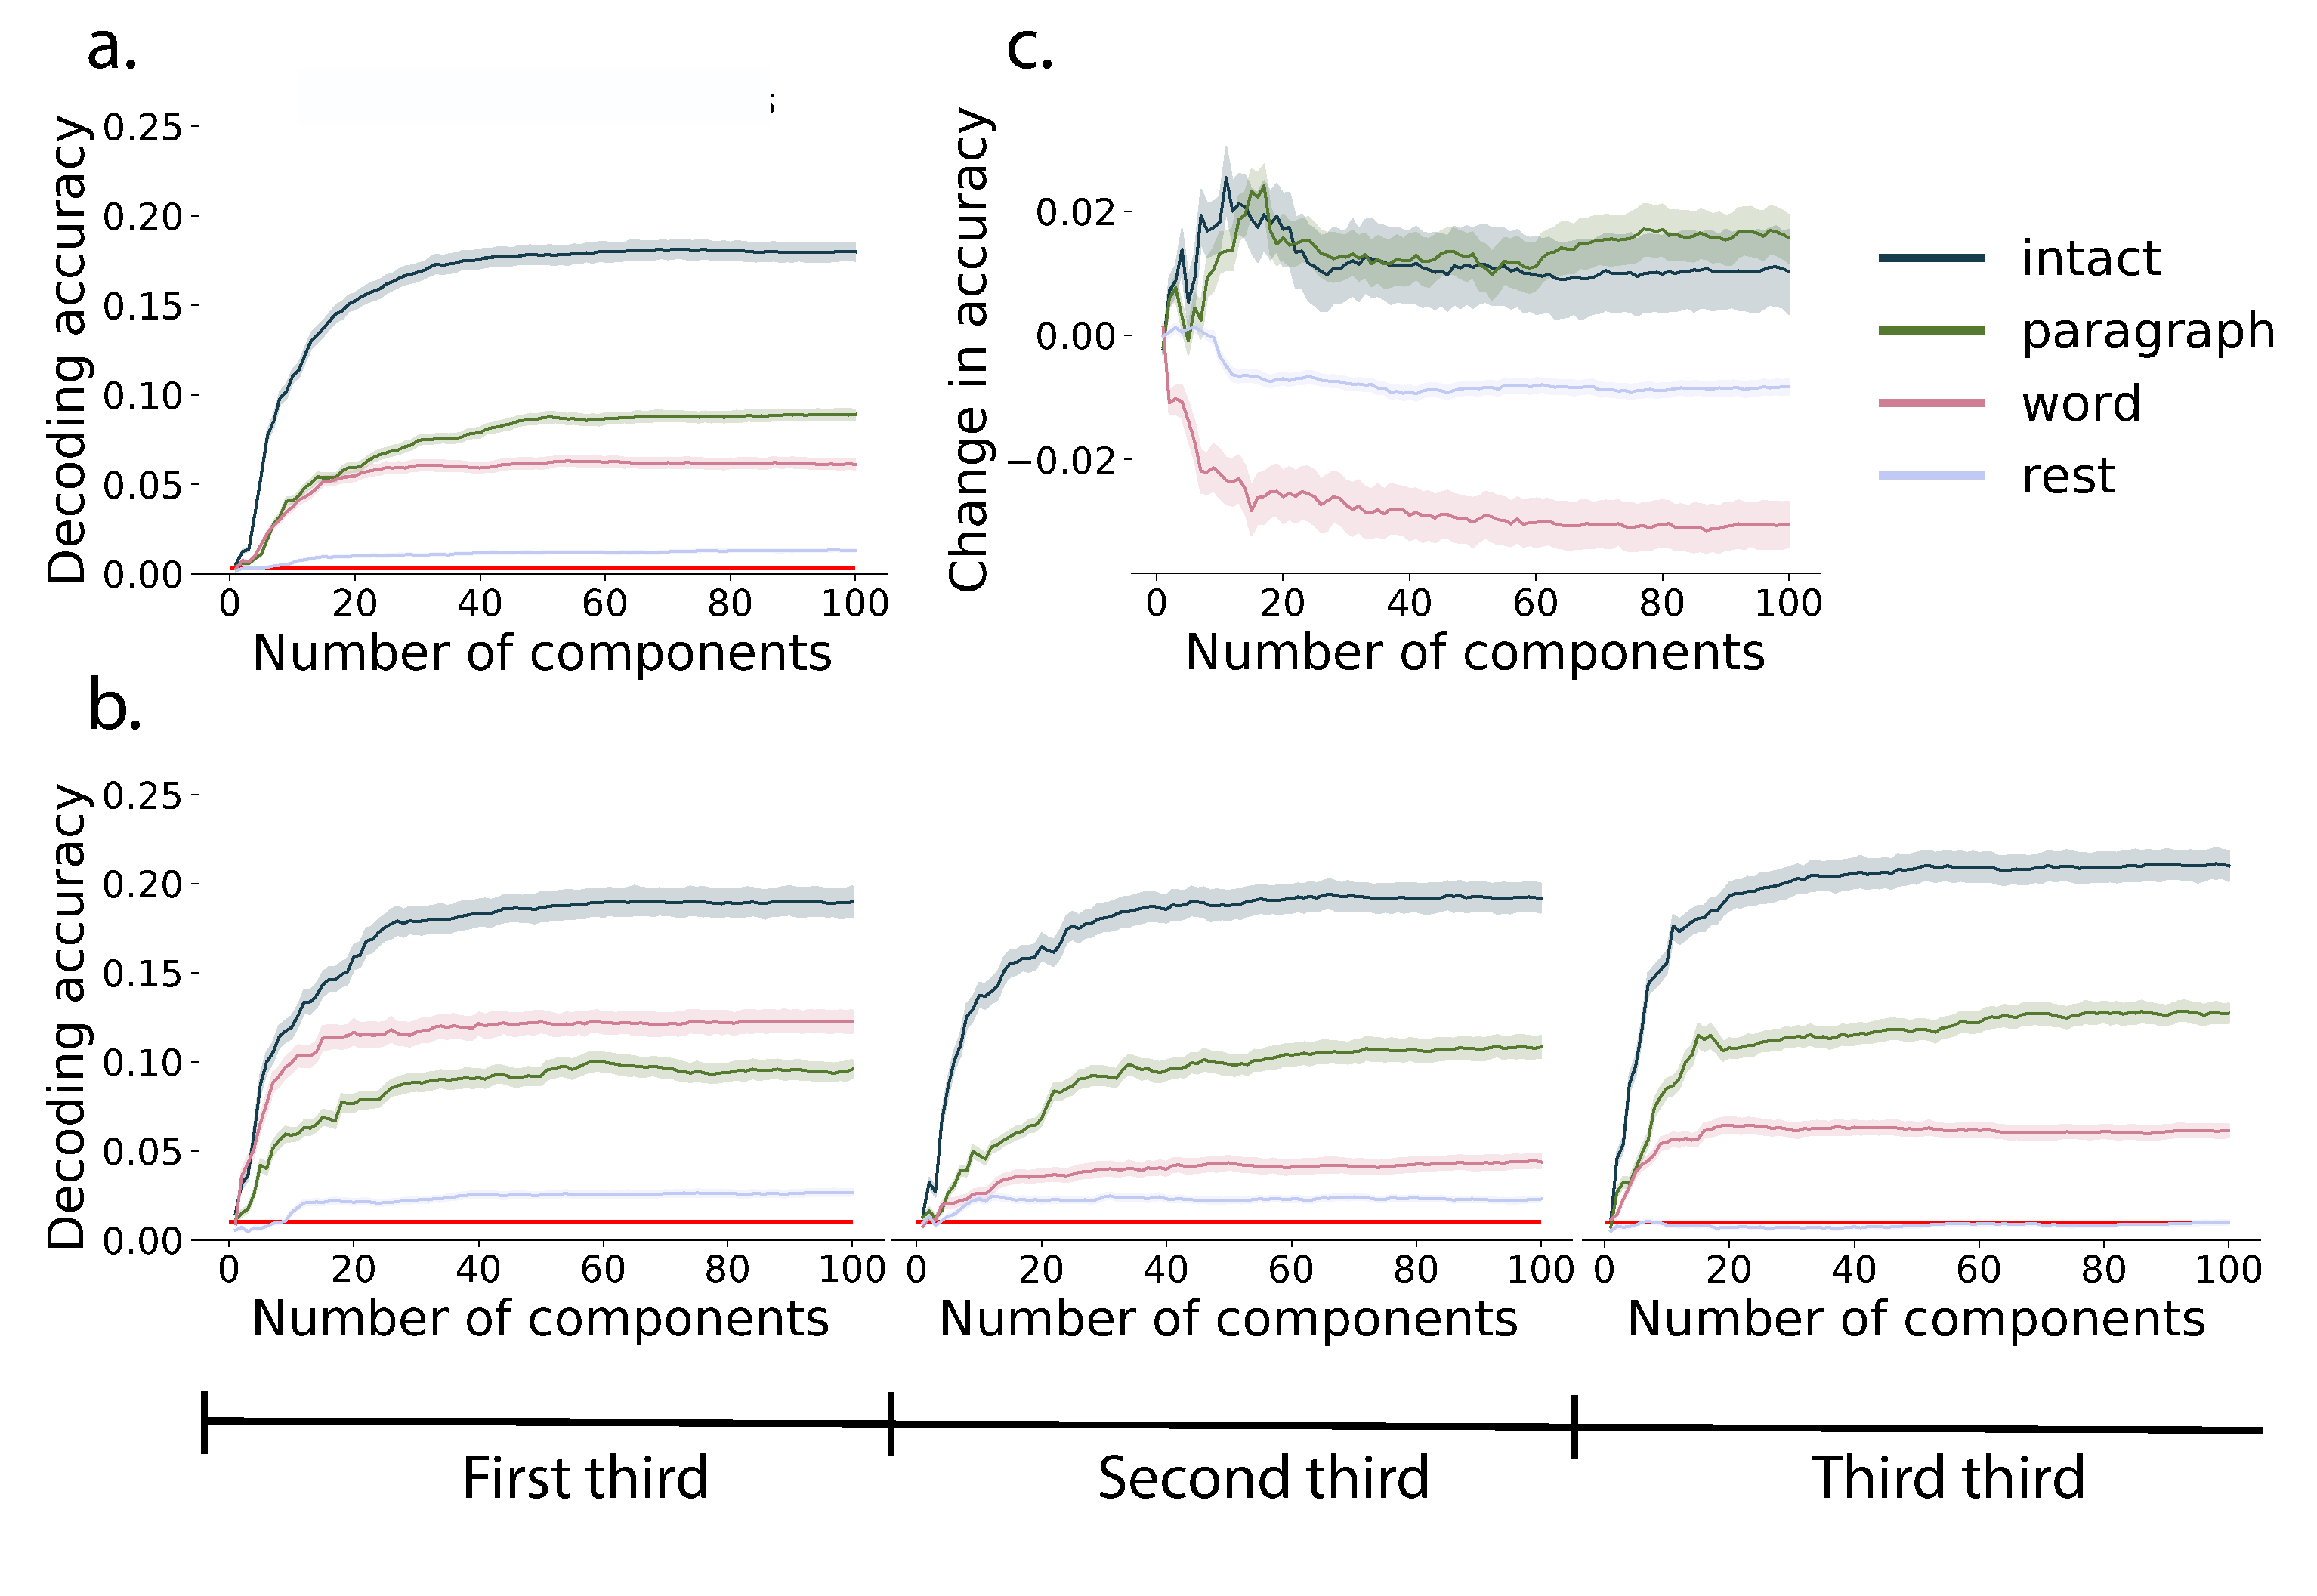
\includegraphics[width=\textwidth]{figs/decode_pcs.pdf}
  \caption{\textbf{Inflection points by thirds.} \textbf{a.}
    Decoding accuracy by number of components not broken into thirds
    (Fig.~\ref{fig:decode_interpret} a.). \textbf{b. and c.}
    Quantifying changes in decoding accuracy across
time. \textbf{b.} Slope of decoding accuracy was calculated by fitting
a regression line for each component/condition for each
third. \textbf{c.}  We also repeated the analysis
(Fig.~\ref{fig:decode_interpret}, b.) to obtain the inflection point
for each condition and for each third. \textbf{d.}  Decoding accuracy by number of components for each third of the scan time. We repeated the same analysis in Fig.~\ref{fig:decode_interpret} a. but breaking the scan time for each condition into 3 intervals.
}
  \label{fig:decode_pcs_thirds}
\end{figure}

We were also curious how compression would change across time.  If, there is some understanding of the narrative that accumulates over time, we should be able to see that difference. We found increases in decoding accuracy with the same number or fewer components for more complex, cognitively rich, conditions.
We also found decreases in decoding accuracy for the word-scrambled and rest
condition.

Overall, we found that as story listening conditions become more complex, more components are required to decode. We also found we could decode better with more impoverished data when
there is the underlying structure of the narrative providing more cognitive richness. We posit that as the complexity of our thoughts increases, neural compression decreases. However, as our thoughts become deeper and richer, more reliable information is available at higher neural compression.



% - Increases in decoding accuracy with the same number or fewer components for more complex, cognitively rich, conditions.
% - Decreases in decoding accuracy for the word-scrambled and rest
% condition.


%%%%%%%%%%%%%%%%%%%%%%%%%%%%%%%%%%%%%%%
\section*{Discussion}


- We trained classifiers using more and more principle components to decode, and compared across condi- tions with varying degrees of cognitive richness.
-We found that as listening conditions become more cognitively rich,
decoding accuracy increased.
-Also, decoding accuracy increased as understanding of the narrative
accumulated over time, in more complex listening conditions.
- Decoding accuracy also increased in higher cognitive areas, in more complex listening conditions.
-We found that as story listening conditions become more complex, more
components are required to decode.
-We also found we could decode better with more impoverished data when
there is the underlying structure of the narrative providing more cognitive richness.
-We posit that as the complexity of our thoughts increases, neural
compression decreases. However, as our thoughts become deeper and richer, more reliable information is available at higher neural compression.







Based on prior work ~\citep{Deme19} and following the direction of the field ~\citep{Turk13} we think our thoughts might be encoded in
dynamic network patterns, and possibly higher order network
patterns (Fig.~\ref{fig:direction_of_field}). We sought to test this hypothesis by developing an approach
to inferring high-order network dynamics from timeseries data. 

One challenge in studying dynamic interactions is the
computational resources required to calculate higher-order correlations. 
We developed a computationally tractable model of network dynamics (Fig.~\ref{fig:methods_fig}) that takes in a feature
timeseries and outputs approximated first-order dynamics (i.e.,
dynamic functional correlations), second-order dynamics
(reflecting homologous networks that dynamically form and disperse),
and higher-order network dynamics (up to tenth-order dynamic
correlations).

We first validated our model using synthetic data, and explored how
recovery varied with different underlying data structures and kernels.   We then 
applied the approach to an fMRI dataset
~\citep{SimoEtal16} in which participants listened to an audio
recording of a story, as well as scrambled versions of the same story
(where the scrambling was applied at different temporal scales).  We
trained classifiers to take the output of the model and decode the
timepoint in the story (or scrambled story) that the participants were
listening to. We found that, during the intact listening condition in the
experiment, classifiers that incorporated higher-order correlations
yielded consistently higher accuracy than classifiers trained only on
lower-order patterns (Fig.~\ref{fig:decoding_level},  a.\&d.).  By contrast, these
higher-order correlations were not necessary to support decoding the other
listening conditions and (minimally
above chance) during a control rest condition.  This suggests
that the cognitive processing that supported the most cogntively rich listening conditions
involved second-order (or higher) network dynamics.

Although we found decoding accuracy was best when incorporating
higher-order network dynamics for all but rest
  condition, it is unclear if this is a product of the brain or the
  data collection technique.  It could be that the brain is
  second-order or it could be that fMRI can
  only reliably give second-order interactions. Exploring this method
  with other data collection technique will be important to
  disentangle this question.



  \subsection*{Concluding remarks}

How can we better understand how brain patterns change over
time? How can we quantify the potential network dynamics that might be
driving these changes? One way to judge the techniques of the future is
to look at the trajectory of the fMRI field so far has taken so far
(Fig.~\ref{fig:methods_fig}).  The field started with 
univariate activation, measuring the average activity for each voxel.
Analyses of multivariate activation followed, looking at spatial patterns of
activity over voxels. Next, correlations of activity were explored, first
with measures like resting connectivity that take temporal correlation
between a seed voxel and all other voxels then with full connectivty
that measure all pairwise correlations.  Additionally, this path of increasing
complexity also moved from static to dynamic measurements.  One
logical next step in this trajectory would be dynamic higher-order
correlations. We have created a method 
to support these calculations by scalably approximating dynamic higher-order
correlations.  

\section*{Acknowledgements}
We acknowledge discussions with Luke Chang, Hany Farid, Paxton
Fitzpatrick, Andrew Heusser, Eshin Jolly, Qiang Liu, Matthijs van der
Meer, Judith Mildner, Gina Notaro, Stephen Satterthwaite, Emily
Whitaker, Weizhen Xie, and Kirsten Ziman. Our work was supported in
part by NSF EPSCoR Award Number 1632738 to J.R.M. and by a sub-award
of DARPA RAM Cooperative Agreement N66001-14-2-4-032 to J.R.M.  The
content is solely the responsibility of the authors and does not
necessarily represent the official views of our supporting
organizations.

\section*{Author contributions}
Concept: J.R.M. and L.L.W.O. Implementation: L.L.W.O., and
J.R.M.  Analyses: L.L.W.O and J.R.M.

\bibliographystyle{apacite}
\bibliography{CDL-bibliography/cdl}

\end{document}


